\section{Frontend - Webapplikation als REST-Client}
\subsection{Überblick}
Das \Gls{backend} muss mit dem \Gls{frontend} verbunden werden.Es gibt unterschiedliche Möglichkeiten dies zu realisieren. Beim Realisieren, muss darauf geachtet werden, dass eine Struktur vorhanden ist. Es werden 2 verschiedene \Gls{designpattern} angeschaut und verglichen. Umgesetzt wird dann ein \Gls{designpattern} mithilfe von \Gls{js}. Hier kann ein \Gls{jsframework} zum Einsatz kommen. Dazu werden hier verschiedene \Gls{jsframework}s angeschaut und verglichen. Für die Verarbeitung der Daten ist es wichtig Datenformate festzulegen. Die Aufbereitung der Elemente fürs \Gls{frontend} mit den Daten des \Gls{backend}s wird ebenfalls angeschaut.
\subsection{Design-Patterns}
Dieser Teil des Projektes wird in Verwendung eines \Gls{designpattern}s umgesetzt. Zwei \Gls{designpattern}s werden hierbei in Betrachtung gezogen. Zum einen \Gls{mvvm} und zum anderen \Gls{mvc}. Es kommen diese zwei Entwurfsmuster in Frage, da \Gls{mvc} in sehr bekanntes \Gls{designpattern} ist und MVVM eine neuere Variante von \Gls{mvc} ist.
\subsubsection{MVC}
\Gls{mvc} ist ein \Gls{designpattern} mit dem eine Software in die drei Teile (Model, View und Controller) geteilt wird.\\\\
Das Model beinhaltet alle Daten der Software und auch alle Funktionen, die mit den Daten interagieren oder mit ihnen rechnen.\\\\
Die View ist der Teil der Software, die Benutzer*innen sehen und mit denen sie interagieren. Dieser Teil der Software beinhaltet keine wichtigen Daten oder Funcktionen, welche Daten bearbeiten. Sie hört nur auf Benutzereingaben und zeigt die bereitgestellten Daten an.\\\\
Der Controller ist der Teil der Software, der Model und View verbindet. In dem Controller wird auf die Benutzereingaben reagiert und die richtigen Funktionen aus dem Model aufgerufen.\cite{mvc}
\begin{figure}[H]
	\centering
	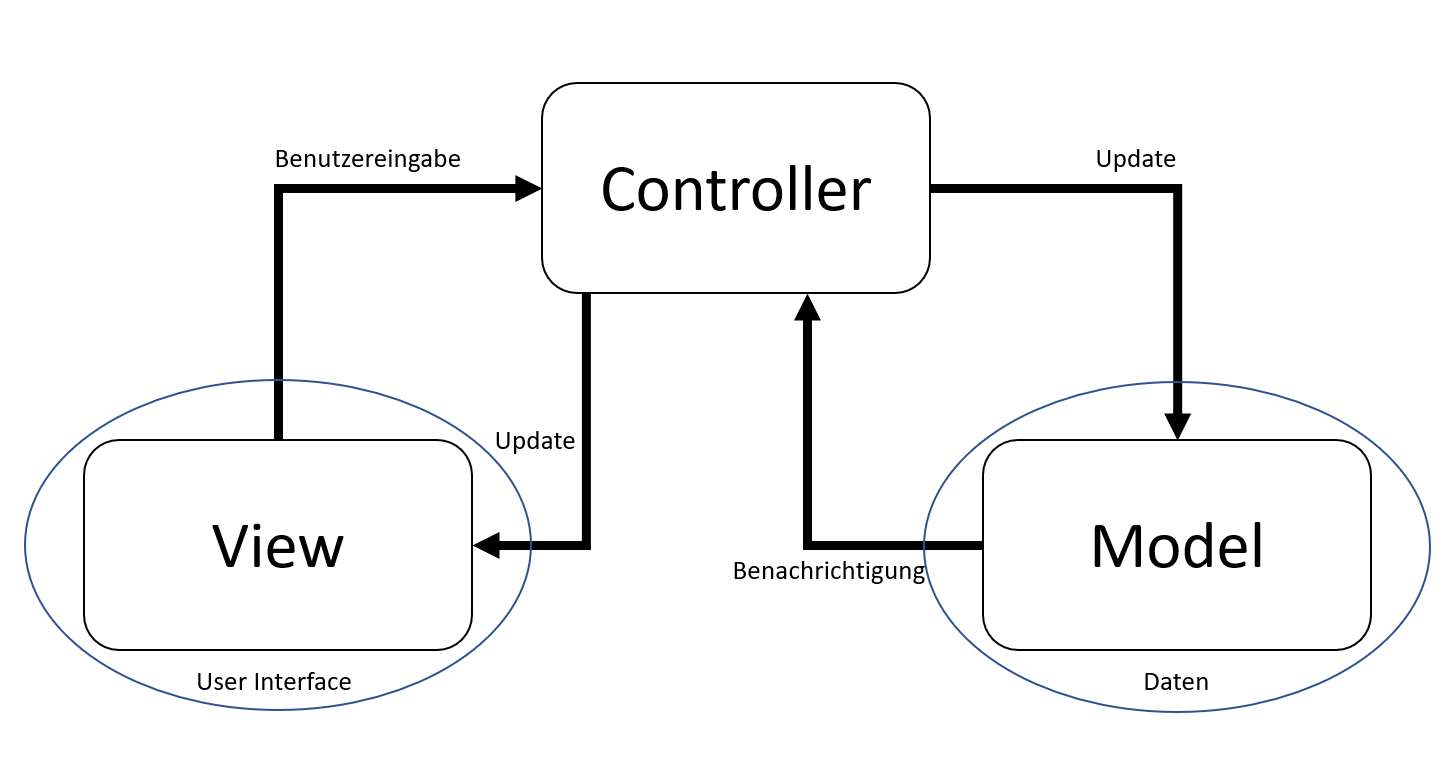
\includegraphics[width=0.8\linewidth]{images/mvc}
	\caption[Übersicht des MVC-Patterns]{Übersicht über die Komponenten des MVC-Patterns und ihre Zusammenhänge}
	\label{fig:mvc}
\end{figure}
\subsubsection{MVVM}
\Gls{mvvm} ist ein \Gls{designpattern} mit dem eine Software in drei Teile geteilt wird. Jedoch wird bei \Gls{mvvm} die Software in Model, View und ViewModel aufgeteilt.\\\\
Das Model beinhaltet wie im konventionellen \Gls{mvc}-Pattern alle wichtigen Daten und Funktionen.\\\\
Die View ist wie beim \Gls{mvc}-Pattern der Teil der Software, mit der Benutzer*innen interagieren.\\\\
Das ViewModel ist ein Bindeglied zwischen Model und View. Dabei stellt es der View offen Funktionen zur Verfügung. Diese können auch Daten verändern bzw. mit Daten rechnen. Das Model kann über das ViewModel auch mit der View direkt interagieren.\cite{mvvm_vue}
\begin{figure}[H]
	\centering
	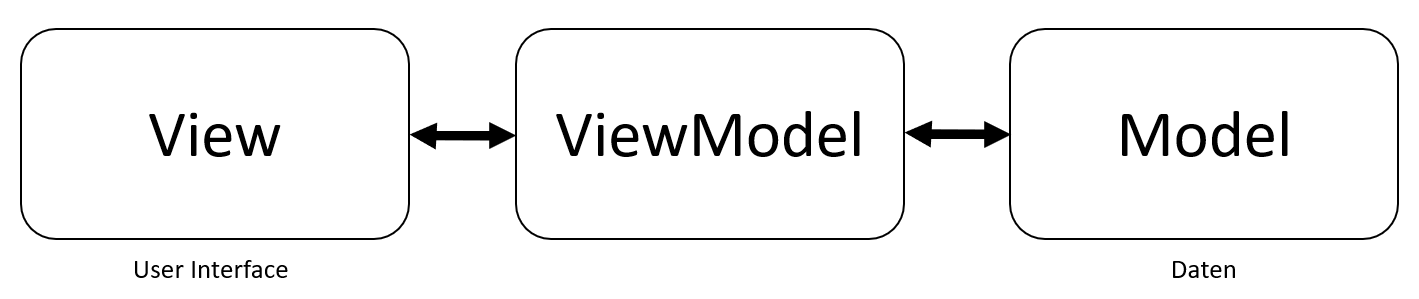
\includegraphics[width=0.8\linewidth]{images/mvvm}
	\caption[Übersicht des MVVM-Patterns]{Übersicht über die Komponenten des MVVM-Patterns und ihre Zusammenhänge}
	\label{fig:mvc}
\end{figure}
\subsubsection{Vergleich}
\subsection{Datenformate}
\subsection{Umsetzungsmöglichkeiten}
\subsubsection{Vue}
\subsubsection{React}
\subsubsection{Angular}
\subsubsection{Ohne Framework}
\subsubsection{Vergleich}
\subsection{Aufbereitung der Daten}
\subsection{Fragestellung}